\documentclass[a4paper]{scrreprt}

%% Language and font encodings
\usepackage[ngerman]{babel}
\usepackage[utf8]{inputenc}
\usepackage[T1]{fontenc}

%% Sets page size and margins
\usepackage[a4paper,top=2.5cm,bottom=2cm,left=2cm,right=2cm]{geometry}

%% Useful packages
\usepackage{amsmath}
\usepackage{graphicx}
\usepackage[colorinlistoftodos]{todonotes}
\usepackage[colorlinks=true, allcolors=blue]{hyperref}

\title{Mr. Trash}
\subtitle{App zur effizienten Müllentsorgung}
\author{
    Hurbean, Alexander\\
    \texttt{e1625747}
    \and
    Schweiger, Phillipp\\
    \texttt{e01634254}}
\titlehead{\centering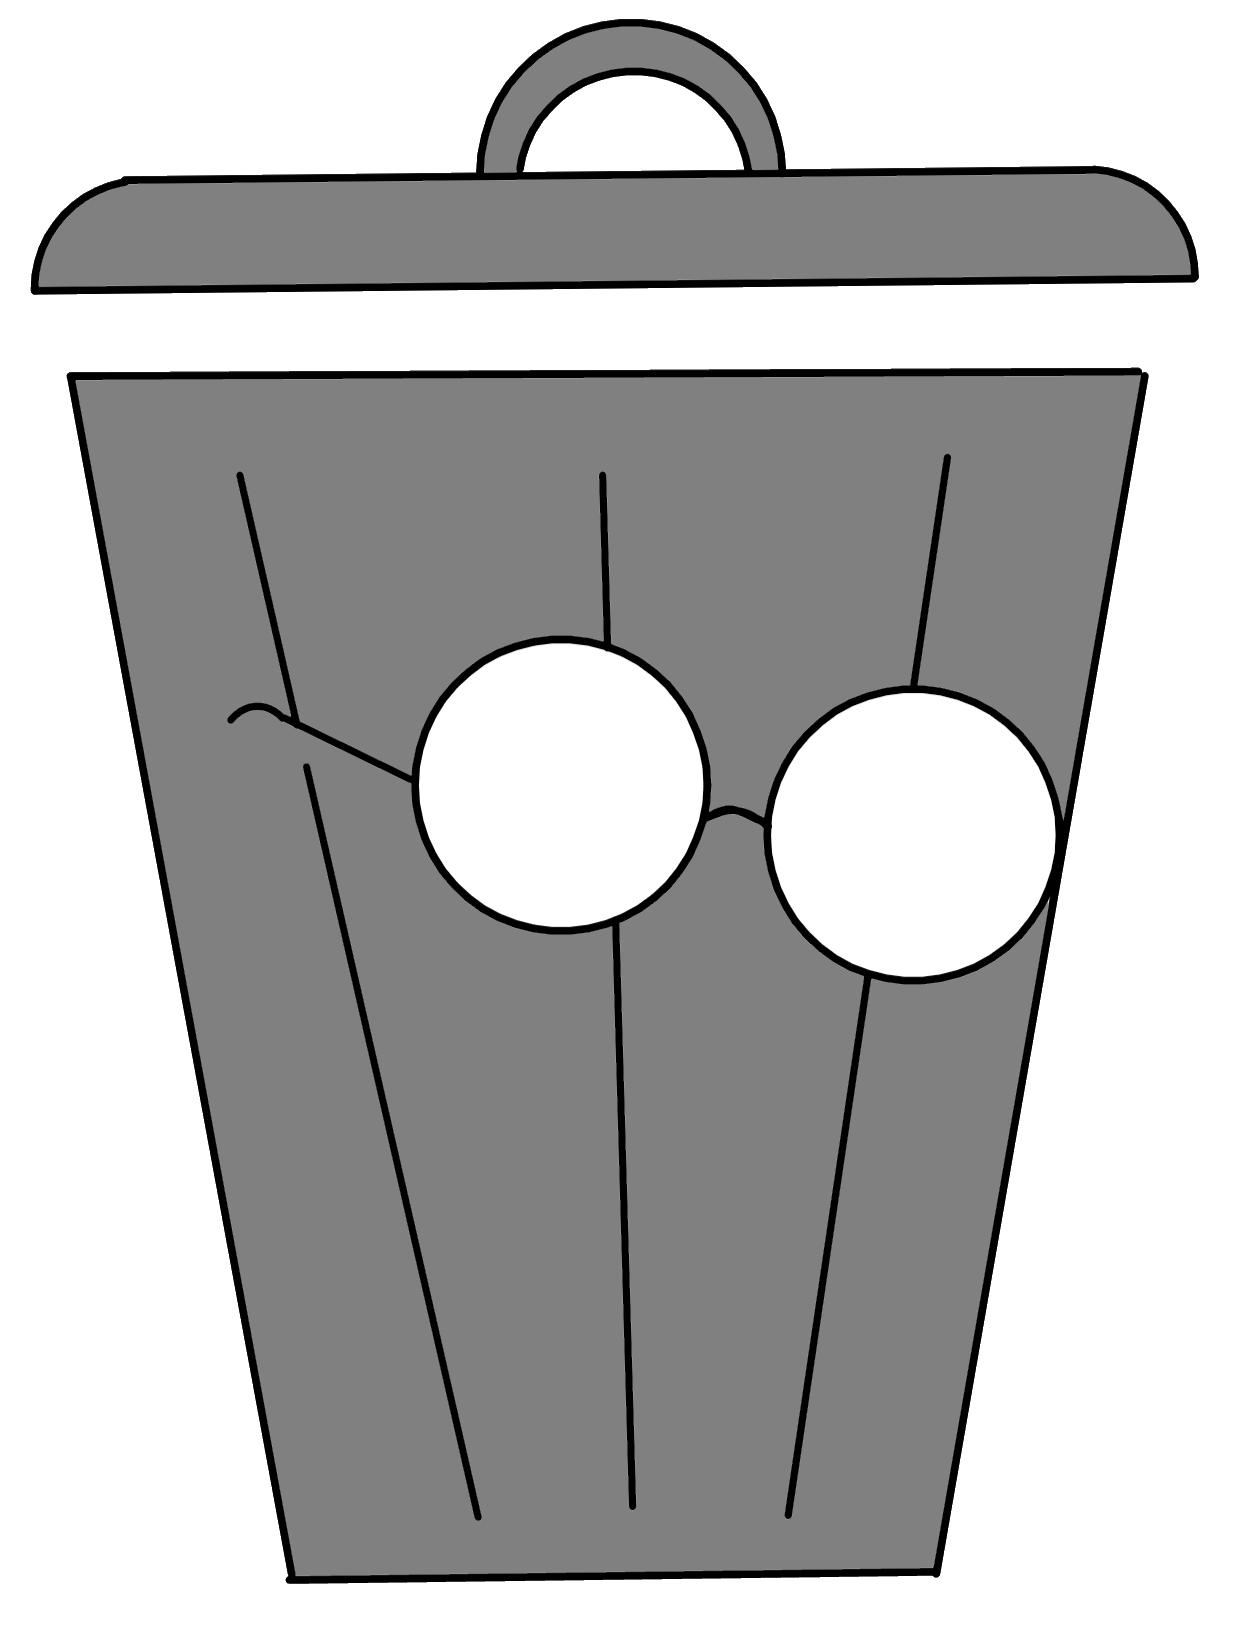
\includegraphics[width=6cm]{../graphical/logo_draft_color.png}}


\begin{document}
\maketitle

\null\vfill
\noindent
App Design Document\\ 
Mobile (App) Software Engineering\\
Technische Universität Wien\\
Version v1.0, März 2019\\
\newpage

%\begin{abstract}
%Short abstract of the game (max 150 words) 
%\end{abstract}

\tableofcontents

% ______________________
% chapter Konzept
% ______________________
\chapter{Konzept}

\section{Kurzbeschreibung}
Mr.Trash ermöglicht es dem unerfahrenen Mülltrenner effizient den richtigen Ort, seinen Müll zu entsorgen, in seiner Nähe zu finden. Die App stellt sicher, dass nie wieder Müll falsch entsorgt wird und somit Umweltfreundlichkeit gewährleistet wird und der Nutzer möglichst wenig Zeit und Know-How benötigt.

\section{Beschreibung der gewählten Datensätze}
\begin{itemize}
	\item Sämtliche Müll-Daten Wien \cite{alleMuell}
	\item Problemstoffsammelstelle Wien \cite{problemstoffsammelstellen}
	\item Altstoffsammelstelle Wien \cite{alstoffsammelstellen}
	\item Mistplätze Standorte Wien \cite{mistplaetze}
	\item Mobile Problemstoffsammelstelle Standorte Wien \cite{mobileProblemstoffsmst}
	\item Christbaumsammelstellen Wien \cite{christbaumsammelstellen}
	\item Mülltrenn ABC \cite{muelltrennabc}
\end{itemize}

% ______________________
% chapter Graphischer Entwurf
% ______________________

\chapter{Graphischer Entwurf} 

\section{High-Fidelity Mockup}
\begin{figure}[h]
\centering

\includegraphics[width=0.3\textwidth]{../graphical/test.jpg}
\caption{\label{fig:art1} Art example}
\end{figure}

\section{Product Icon}
\begin{figure}[h]
\centering
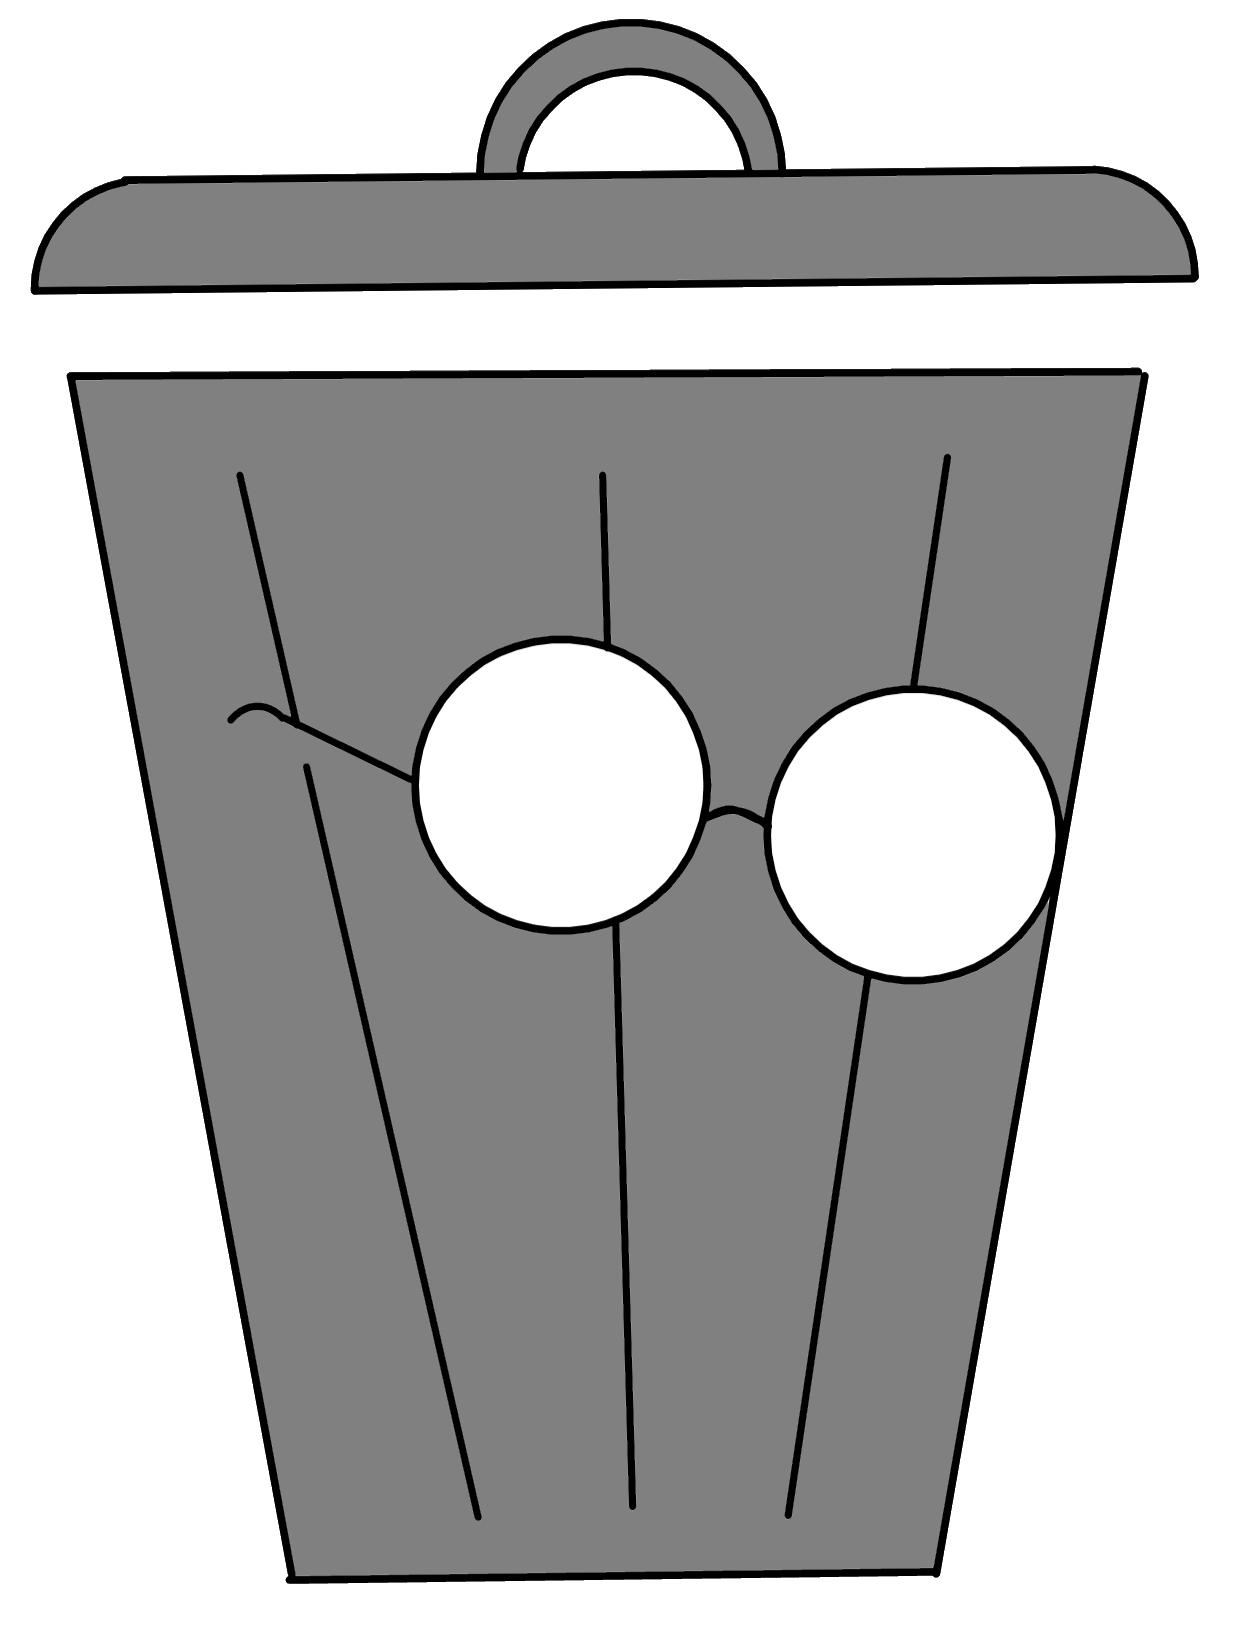
\includegraphics[width=0.3\textwidth]{../graphical/logo_draft_color.jpg}
\caption{\label{fig:art2} Art example}
\end{figure}

\bibliographystyle{abbrv}
\bibliography{references}

\end{document}